% ---------------------------------------------------------------------------
% Figure 1 + Table 1 side by side, each with its caption, in two minipages of
% exactly the same height. The table (caption on top) sets the height; the figure
% box gets whatever height its own caption leaves over, and the image is centred
% in that box. Both captions are typeset once into boxes, so what is measured is
% exactly what is placed.
% Needs: graphicx, booktabs, caption. Files: table1.tex, figure1.pdf.
% The log prints "FIGBOX: width=..., height=..." -- re-render figure1.pdf at that
% size (src/fig1.py <width_pt> <height_pt>) if the template changes the box size.
% ---------------------------------------------------------------------------
\newsavebox{\tblbox}\newsavebox{\figcapbox}
\newlength{\tblH}\newlength{\figcapH}\newlength{\figH}
\newcommand{\figW}{0.37\linewidth}
\newcommand{\tblW}{0.61\linewidth}
\newcommand{\figcaptext}{Who keeps beating their points. Next-season wins above the points-based expectation by quintile
of UPR+ and of the official rating (508 player-seasons; adjusted for points won, ranking, age, volume, season; 95\% CI).}
\begin{figure}[b]
\footnotesize
\sbox{\tblbox}{\begin{minipage}[b]{\tblW}
% Table 1 -- requires booktabs and caption (\captionof, \captionsetup); place inside a minipage.
\captionsetup{position=above}
\captionof{table}{Official Under Pressure components vs.\ UPR+. Reliability: the same charted matches, 158 players with
$\geq$20 (median 46); split-half $r$ (odd vs.\ even matches), matches needed for reliability 0.5, correlation with points won.
Prediction: 508--536 player-seasons; effect of 1 SD over the three prior seasons on next-season wins above the points-based
expectation (pp per match) and ranking (\%), adjusted for points won, ranking, age, volume and season; 95\% CI.}
\label{tab:uprplus}
\centering
\setlength{\tabcolsep}{2.2pt}\renewcommand{\arraystretch}{1.04}
\begin{tabular*}{\linewidth}{@{\extracolsep{\fill}}lrrrrr@{}}
\toprule
 & \multicolumn{3}{c}{Reliability} & \multicolumn{2}{c}{Next season, per SD} \\
\cmidrule(lr){2-4}\cmidrule(l){5-6}
 & Split- & Matches & $r$ with & Wins vs. & Ranking \\
Signal & half $r$ & to 0.5 & skill & points (pp) & (\%) \\
\midrule
Break points saved & 0.34 & 34 & 0.48 & $+0.30$ & $-2.7$ \\
Break points converted & 0.18 & 42 & 0.38 & $-0.21$ & $+2.1$ \\
Tiebreaks won & $-0.02$ & 612 & 0.35 & $+0.15$ & $+0.4$ \\
Deciding sets won & 0.06 & 119 & 0.30 & $+0.38$ & $+3.7$ \\
Official UPR (sum) & 0.14 & 144 & 0.53 & $+0.48$ & $+1.6$ \\
\textbf{UPR+} & \textbf{0.26} & \textbf{55} & 0.31 & $\mathbf{+1.01}$ & $-4.3$ \\
 & & & & {\scriptsize[0.64, 1.39]} & {\scriptsize[$-11.6$, 3.6]} \\
\bottomrule
\end{tabular*}

\par\vspace{0pt}\end{minipage}}%
\setlength{\tblH}{\dimexpr\ht\tblbox+\dp\tblbox\relax}%
\sbox{\figcapbox}{\begin{minipage}[t]{\figW}\captionsetup{position=below}\captionof{figure}{\figcaptext}\label{fig:quint}\end{minipage}}%
\setlength{\figcapH}{\dimexpr\ht\figcapbox+\dp\figcapbox\relax}%
\setlength{\figH}{\dimexpr\tblH-\figcapH\relax}%
\typeout{FIGBOX: width=\the\dimexpr\figW\relax, height=\the\figH, total=\the\tblH}%
\begin{minipage}[b][\tblH][t]{\figW}
\parbox[b][\figH][c]{\linewidth}{\centering
  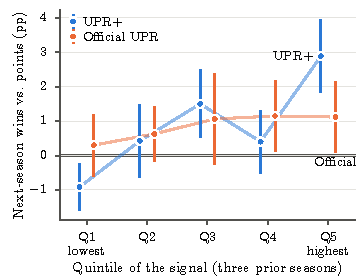
\includegraphics[width=\linewidth,height=\figH,keepaspectratio]{figure1.pdf}}\par\nointerlineskip
\usebox{\figcapbox}
\end{minipage}\hfill
\usebox{\tblbox}
\end{figure}
